% !TEX root = /Users/vinicius/projects/latex/ee522/main.tex
\documentclass[12pt]{article}
\author{
  Vitor Bergamaschi Dos Santos - 248212\\
  Vinicius De Lima Quadrado - 225357\\
  Leonardo Souza Boaventura - 250417
}
% Pacotes básicos
\usepackage[utf8]{inputenc}
\usepackage[T1]{fontenc}
\usepackage[brazil]{babel}
\usepackage{graphicx}
\usepackage{amsmath, amssymb}
\usepackage{caption}
\usepackage{float}
\usepackage{geometry}
\usepackage{booktabs}
\usepackage{hyperref}
\geometry{a4paper, margin=2.5cm}
\usepackage{indentfirst}
\usepackage{subcaption}
\usepackage[section]{placeins}
\usepackage{float}
\usepackage{pgfplots}
\pgfplotsset{compat=newest}
\usepackage{booktabs}

\title{\textbf{Relatório de Laboratório -- EE522}}
\date{\textbf{EXPERIMENTO IV:} Crosstalk
\\ \textbf{Data:} 30/05/2025}

\begin{document}

\maketitle

\section{Objetivos}
Nas seções abaixo seguem os objetivos de cada seção do experimento.

\subsection{Crosstalk}
Nesta seção será tratada a interferência de campos elétricos e
magnéticos entre trilhas de circuito impresso, também conhecido como
crosstalk, avaliando a influência da distância e da orientação entre
as trilhas na indução de tensão em trilhas e circuitos vizinhos.
Também será comparada a diferença na tensão induzida quando usado
sinais de ondas senoidais e quadradas, em diferentes frequências.
Por fim discutiremos a razão do ganho de tensão em função da
frequência para três circuitos, dentre eles dois com trilhas
paralelas e outro com trilhas perpendiculares.

\subsection{Casamento de impedância}
Será discutido o fenômeno de reflexão de sinais em linhas de
transmissão e com isso avaliar a importância do casamento de
impedâncias entre fonte, linha e carga. Iremos observar também que
existem situações em que o casamento de impedância é desejado ou indesejado.

\section{Procedimento Experimental}
Nas seções abaixo seguem os procedimentos experimentais de cada seção
do experimento.

\subsection{Seção I - Crosstalk em Placa de Circuito Impresso}

Abaixo seguem as seções que descrevem a montagem, equipamentos
utilizados e procedimento de execução do Crosstalk em Placa de
Circuito Impresso.

\subsubsection{Montagem}
Utilizou-se a placa com esquemático mostrado na figura \ref{fig:img/pcb-esquema.png}, com quatro
trilhas, uma de alimentação (A), P1, P2 e P$\perp$.
As trilhas com orientação paralela em relação a trilha A são as
trilhas P1 e P2, com distância entre A de 1 e 2 milímetros,
respectivamente. A trilha perpendicular a A é a trilha P$\perp$.

\begin{figure}[H]
  \centering
  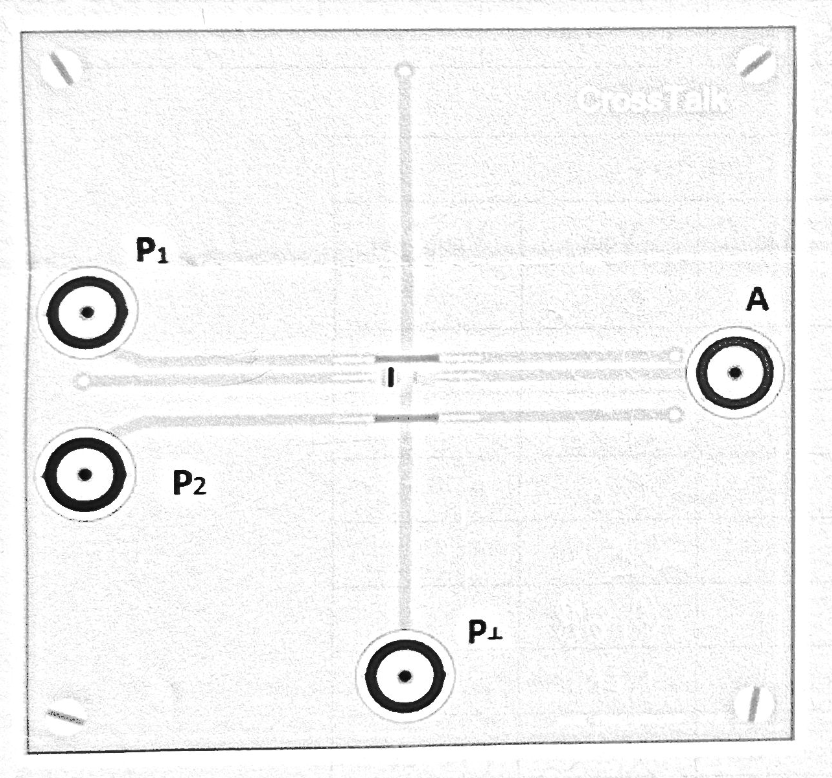
\includegraphics[width=0.8\textwidth]{img/pcb-esquema.png}
  \caption{Esquemático da placa de circuito impresso utilizada no experimento}
  \label{fig:img/pcb-esquema.png}
\end{figure}

Liga-se o gerador de sinais ao conector A e liga-se a trilha de
interesse ao osciloscópio, ambas conexões são feitas via cabo coaxial.

\subsubsection{Equipamentos utilizados}
Foram usados um gerador de sinais configurado com output de 10 Vpp e
frequência variável, um osciloscópio, dois cabos coaxiais e uma placa
de circuito impresso customizada.

\subsubsection{Execucao}
Fixou-se a nível da tensão de entrada em 10Vpp, e iniciamos o
processo de aumentar a frequência do gerador em conectado a trilha A.
Para cada trilha de medição (p1, p2, P$\perp$) foi colhido o valor
vpp da tensão induzida dada uma frequência definida.
Na sequência medimos também a tensão induzida em P1 e P$\perp$ para o
caso de onda quadrada, em função de um rol menor de frequências.
Por fim calculou-se a razão do ganho de tensão (mod(Vout;Vin)) para
cada ponto de cada circuito.

\subsection{Seção II - Casamento de Impedâncias / Reflexão de Sinais
em Linhas de Transmissão}

Abaixo seguem as seções que descrevem a montagem, equipamentos
utilizados e procedimento de execução do experimento de Casamento de
Impedâncias e Reflexões de Sinais em Linhas de Transmissão.

\subsubsection{Montagem}
[placeholder]

\subsubsection{Equipamentos utilizados}
[placeholder]

\subsubsection{Execucao}
[placeholder]

\section{Resultados}
Nas seções abaixo seguem as discussões dos resultados de cada seção
do experimento.

\subsection{Seção I -  Crosstalk em Placa de Circuito Impresso}
Nestas seções apresentaremos os dados, os equipamentos utilizados e o
método de execução desta seção

\subsubsection{Apresentação de dados}

Os gráficos \ref{fig:ganho-frequencia-p1}, \ref{fig:ganho-frequencia-p2} e
\ref{fig:ganho-frequencia-pperp} representam respectivamente os ganhos de
tensão de entrada em A e tensão induzida em P1, P2 e P$\perp$, em função da
frequência da tensão de entrada. As tabelas dos dados obtidos no
experimento estão disponíveis no anexo A.

Já a tabela \ref{tab:ganho-onda-quadrada} mostra os ganhos de tensão
de entrada em A e tensão induzida em P1 e P$\perp$, para o caso de
onda quadrada, em três frequências distintas.

\begin{figure}[H]
  \captionsetup{name=Gráfico}
  \centering
  \begin{tikzpicture}
    \begin{loglogaxis}[
        xlabel={Frequência $kHz$},
        ylabel={Ganho $V_o/V_i$},
        grid=both,
        minor tick num=9,
        width=10cm,
        height=8cm,
        mark size=2pt,
        tick label style={/pgf/number format/fixed},
        log ticks with fixed point,
      ]
      \addplot[
        only marks,
        mark=*,
        blue
      ] table[row sep=\\] {
        x y \\
        50 0.11818\\
        200 0.29091\\
        400 0.92727\\
        1000 1.14545\\
        2000 1.85455\\
        4000 3.45455\\
        8000 6.18182\\
        10000 7.70909\\
      };
    \end{loglogaxis}
  \end{tikzpicture}
  \caption{Ganho em função da frequência para o circuito P1}
  \label{fig:ganho-frequencia-p1} % <-- Aqui está o lugar certo!
\end{figure}

\begin{figure}[H]
  \captionsetup{name=Gráfico}
  \centering
  \begin{tikzpicture}
    \begin{loglogaxis}[
        xlabel={Frequência $kHz$},
        ylabel={Ganho $V_o/V_i$},
        title={Ganho em função da frequência - Circuito P2},
        grid=both,
        minor tick num=9,
        width=10cm,
        height=8cm,
        mark size=2pt,
        tick label style={/pgf/number format/fixed},
        log ticks with fixed point,
      ]
      \addplot[
        only marks,
        mark=*,
        blue
      ] table[row sep=\\] {
        x y \\
        50      0.07273 \\
        200      0.10182 \\
        400      0.20364 \\
        1000  0.39273 \\
        2000  0.71273 \\
        4000  1.63636 \\
        8000  2.87273 \\
        10000  3.56364 \\
      };
    \end{loglogaxis}
  \end{tikzpicture}
  \caption{Ganho em função da frequência para o circuito P2}
  \label{fig:ganho-frequencia-p2} % <-- Aqui está o lugar certo!
\end{figure}

\begin{figure}[H]
  \captionsetup{name=Gráfico}
  \centering
  \begin{tikzpicture}
    \begin{loglogaxis}[
        xlabel={Frequência $kHz$},
        ylabel={Ganho $V_o/V_i$},
        grid=both,
        minor tick num=9,
        width=10cm,
        height=8cm,
        mark size=2pt,
        tick label style={/pgf/number format/fixed},
        log ticks with fixed point,
      ]
      \addplot[
        only marks,
        mark=*,
        blue
      ] table[row sep=\\] {
        x y \\
        50  0.02545 \\
        200  0.02727 \\
        400  0.05091 \\
        800  0.05455 \\
        1000  0.09091 \\
        2000  0.11636 \\
        4000  0.12727 \\
        8000  0.24727 \\
        10000  0.31273 \\
      };
    \end{loglogaxis}
  \end{tikzpicture}
  \caption{Ganho em função da frequência para o circuito P$\perp$}
  \label{fig:ganho-frequencia-pperp} % <-- Aqui está o lugar certo!
\end{figure}

\begin{table}[htbp]
  \centering
  \begin{tabular}{c|cc|cc}
    \toprule
    \textbf{freq (kHz)} & \multicolumn{2}{c|}{\textbf{Circuito P1}} &
    \multicolumn{2}{c}{\textbf{Circuito P}} \\
    & $V_{in}$ & $V_{out}$ (mV) & $V_{in}$ & $V_{out}$ (mV) \\
    \midrule
    50      & 11   & 1.5   & 10 & 0.24 \\
    1000    & 11   & 21.6  & 10 & 20   \\
    10000   & 11   & 200   & 10 & 30   \\
    \bottomrule
  \end{tabular}
  \caption{Ganho em função da frequência - Onda Quadrada}
  \label{tab:ganho-onda-quadrada}
\end{table}

\subsubsection{Análise qualitativa}
A lei de Faraday \ref{eq:lei-faraday} nos diz que a força
eletromotriz induzida em um circuito
fechado é igual ao negativo da variação no tempo do fluxo magnético através da
área limitada pelo circuito fechado.

\begin{equation}
  \label{eq:lei-faraday}
  \oint \vec{E} \cdot d\vec{l} = -\iint \frac{d\vec{B}}{dt}   \cdot d\vec{S}
\end{equation}

Com isto verificamos que a tensão induzida (força eletromotriz) na
bobina dos circuitos P1, P2 e P$\perp$ é diretamente proporcional ao  fluxo
magnético que as atravessa. O campo magnético gerado pela corrente
que está no circuito fechado A gera o fluxo magnético necessário para
ocorrer a indução magnética.

Através dos resultados obtidos, nota-se que a proximidade entre
bobinas A e P1 ou A e P2 é inversamente proporcional à tensão
induzida: P1 com distanciamento de 1mm de A possui maior tensão
induzida que P2 com distanciamento de 2mm de A.

Também como resultado do experimento, notou-se maior ganho de tensão
conforme o aumento da frequência de alimentação, e isso está previsto
na Lei de Faraday. O fluxo magnético cresce quando a variação do
campo magnético cresce, então aumentar a frequência causa a derivada
temporal do campo magnético aumentar. Por isso, em todos os casos
vistos a tensão induzida é sempre maior quando a frequência é maior.

A Lei de Faraday da forma enunciada acima prevê que o circuito
fechado descrito esteja perpendicular à direção do fluxo magnético.
Todavia, quando temos um fluxo magnético em direção qualquer, o dA é
multiplicado pelo cosseno do ângulo entre a direção do fluxo
magnético e o vetor de área de A, vemos isso na equação
\ref{eq:lei-faraday-angulo}.

\begin{equation}
  \label{eq:lei-faraday-angulo}
  \oint \vec{E} \cdot d\vec{l} = -\iint \frac{d\vec{B}}{dt}   \cdot
  d\vec{S} \cdot \cos(\theta)
\end{equation}

Então foi montada uma espira perpendicular a outra, portanto
theta=90graus, o cosseno de theta é nulo e temos uma tensão induzida
nula, segundo a Lei de Faraday.

Através dos resultados obtidos com as bobinas A e P$\perp$ notamos uma
tensão induzida baixíssima e proporcional a frequência. Apesar do
resultado esperado ser tensão induzida nula, temos que levar em
consideração que as bobinas não estão perfeitamente perpendiculares e
isso é suficiente para induzir tensão em P$\perp$.

Por fim testamos os circuitos P1 e P$\perp$ com ondas quadradas nas
frequências de 50, 1000 e 10.000 KHz, em ambos os casos tivemos um
ganho de tensão substancialmente maior do que para as ondas
senoidais. Isso se deve a termos variações abruptas no sinal, na
região de degrau da onda, onde temos uma maior derivada temporal da
corrente em A, consequentemente uma maior derivada do campo magnético
e um maior fluxo de campo magnético.

\subsubsection{Conclusão parcial}

Conclui-se que a proximidade de trilhas em uma placa de circuito
impresso geram tensão induzida nas trilhas vizinhas, e que a tensão
induzida é proporcional a frequência de operação e inversamente
proporcional à distância, logo devemos projetar placas de circuito
impresso que levem em consideração estes fatores.

\subsection{Seção II - Casamento de Impedâncias / Reflexão de Sinais
em Linhas de Transmissão}
Nestas seções apresentaremos os dados, os equipamentos utilizados e o
método de execução desta seção

\subsubsection{Apresentação de dados}
[placeholder]

\subsubsection{Análise qualitativa}
[placeholder]

\subsubsection{Conclusão parcial}
[placeholder]

\section{Conclusão}
[placeholder]

\section{Bibliografia}
WIKIPÉDIA. Lei de Faraday-Neumann-Lenz. Disponível em:
\url{https://pt.wikipedia.org/wiki/Lei_de_Faraday-Neumann-Lenz } .
Acesso em: 29/05/2025.

% UNIVERSIDADE ESTADUAL DE CAMPINAS. Formulário do Experimento IV -
% Ruído Produzido em Chaves Mecânicas Devido a Indutância das Cargas. 2025

\clearpage % Garante quebra de página
\appendix  % Inicia a seção de anexos (muda numeração, se for artigo)

\section*{Anexo A - Tabelas de dados do experimento de Crosstalk}
\addcontentsline{toc}{section}{Anexo A - Tabelas de dados do
experimento de Crosstalk}



\begin{table}[h]
  \centering
  \begin{tabular}{c|c|c|c}
    \toprule
    \textbf{Frequência (kHz)} & \textbf{$V_{in}$ (mV)} &
    \textbf{$V_{in}$ (mV)} & \textbf{${V_{out}}/{V_{in}}$} \\
    \midrule
    50	&11	&1.3	&0.11818 \\
    200	&11	&3.2	&0.29091 \\
    400	&11	&10.2	&0.92727 \\
    1000	&11	&12.6	&1.14545 \\
    2000	&11	&20.4	&1.85455 \\
    4000	&11	&38	&3.45455 \\
    8000	&11	&68	&6.18182 \\
    10000	&11	&84.8	&7.70909 \\
    \bottomrule
  \end{tabular}
  \caption{Ganho de tensão induzida em P1 por A}
  \label{tab:ganho-tensao-p1}
\end{table}

\begin{table}[h]
  \centering
  \begin{tabular}{c|c|c|c}
    \toprule
    \textbf{Frequência (kHz)} & \textbf{$V_{in}$ (mV)} &
    \textbf{$V_{in}$ (mV)} & \textbf{${V_{out}}/{V_{in}}$} \\
    \midrule
    50	&11	&0.8	&0.07273 \\
    200	&11	&1.12	&0.10182 \\
    400	&11	&2.24	&0.20364 \\
    1000	&11	&4.32	&0.39273 \\
    2000	&11	&7.84	&0.71273 \\
    4000	&11	&18	&1.63636 \\
    8000	&11	&31.6	&2.87273 \\
    10000	&11	&39.2	&3.56364 \\
    \bottomrule
  \end{tabular}
  \caption{Ganho de tensão induzida em P2 por A}
  \label{tab:ganho-tensao-p2}
\end{table}

\begin{table}[h]
  \centering
  \begin{tabular}{c|c|c|c}
    \toprule
    \textbf{Frequência (kHz)} & \textbf{$V_{in}$ (mV)} &
    \textbf{$V_{in}$ (mV)} & \textbf{${V_{out}}/{V_{in}}$} \\
    \midrule
    50    &11  &0.28  &0.02545 \\
    200    &11  &0.3    &0.02727 \\
    400    &11  &0.56  &0.05091 \\
    800    &11  &0.6    &0.05455 \\
    1000  &11  &1      &0.09091 \\
    2000  &11  &1.28  &0.11636 \\
    4000  &11  &1.4    &0.12727 \\
    8000  &11  &2.72  &0.24727 \\
    10000  &11  &3.44  &0.31273 \\
    \bottomrule
  \end{tabular}
  \caption{Ganho de tensão induzida em P$\perp$ por A}
  \label{tab:ganho-tensao-pperp}
\end{table}

\end{document}
